\documentclass{beamer}

\usepackage{beamerthemesplit}
\usepackage{verbatim}
\usepackage[normalem]{ulem}
\usepackage[caption=false]{subfig}
%\usepackage{tabularx}
%\usepackage{booktabs}



\usepackage{xcolor}

\usepackage{hyperref}

\definecolor{gold}{rgb}{1.,0.84,0.}
\definecolor{brightred}{rgb}{1.,0.4,0.4}
\definecolor{mygray}{RGB}{200,200,200}
\definecolor{lightsteelblue}{RGB}{176,196,222}
\definecolor{lightskyblue}{RGB}{135,206,250}
\definecolor{cadetblue}{RGB}{95,158,160}

\usetheme{default}
\usecolortheme{mule}

\usefonttheme{serif}

%\DeclareGraphicsExtensions{.pdf,.png,.jpg}

\newcommand{\mcal}{\textsc{metacalibration}}
\newcommand{\Mcal}{\textsc{Metacalibration}}

\newcommand{\mcalR}{\mbox{\boldmath $R$}}
\newcommand{\mcalRscalar}{\mbox{$R$}}

\newcommand{\mcalRmean}{\mbox{\boldmath $\langle R \rangle$}}
\newcommand{\mcalRscalarmean}{\mbox{$\langle R \rangle$}}

\newcommand{\mcalRpsf}{$R^{p}$}
\newcommand{\mcalRpsfnoise}{$R^{p}_\eta$}
\newcommand{\mcalRo}{\mbox{\boldmath $R_o$}}
\newcommand{\mcalRnoise}{\mbox{\boldmath $R_\eta$}}

\newcommand{\mcalRmeanalpha}{\mbox{\boldmath $\langle R_\alpha \rangle$}}
\newcommand{\mcalRmeanbeta}{\mbox{\boldmath $\langle R_\beta \rangle$}}

\newcommand{\mcalRg}{\mbox{\boldmath $R_\gamma$}}
\newcommand{\mcalRS}{\mbox{\boldmath $R_S$}}
\newcommand{\mcalRgmean}{\mbox{\boldmath $\langle R_\gamma \rangle$}}
\newcommand{\mcalRSmean}{\mbox{\boldmath $\langle R_S \rangle$}}

\newcommand{\mcalRtwopt}{\mbox{\boldmath $R^{2pt}$}}
\newcommand{\mcalRtwoptmean}{\mbox{\boldmath $\langle R^{2pt} \rangle$}}


\newcommand{\mcalRmodel}{\mbox{\boldmath $R^{model}$}}
\newcommand{\mcalRnoisemodel}{\mbox{\boldmath $R^{model}_\eta$}}


\newcommand{\vecg}{\mbox{\boldmath $\gamma$}}
\newcommand{\vest}{\mbox{\boldmath $e$}}

\newcommand{\snr}{$S/N$}
\newcommand{\snT}{$(S/N)_{\textrm{size}}$}
%\newcommand{\snT}{$\left( \frac{S}{N}\right)_{\textrm{size}}$}
\newcommand{\snflux}{$(S/N)_{\textrm{flux}}$}
%\newcommand{\snflux}{$\left( \frac{S}{N}\right)_{\textrm{flux}}$}
\newcommand{\hlr}{$r_{50}$}

\newcommand{\neff}{$n_{eff}$}

\newcommand{\lensfit}{\texttt{LENSFIT}}
\newcommand{\numba}{\texttt{Numba}}
\newcommand{\python}{\texttt{Python}}
\newcommand{\ngmix}{\texttt{ngmix}}
\newcommand{\ngmixer}{\texttt{ngmixer}}
\newcommand{\shear}{{\bf g}}
\newcommand{\redmapper}{redMaPPer}
\newcommand{\est}{$e$}


\newcommand{\prelim}{{\bf{\it Preliminary}}}

\newcommand{\uberseg}{{\color{lightsteelblue} {\"u}berseg}}
\newcommand{\MOF}{{\color{brightred}MOF}}


\title{Shear-dependent Detection Biases}
\author{Erin Sheldon}
\institute{Brookhaven National Laboratory}

% http://texblog.net/latex-archive/plaintex/beamer-footline-frame-number/
% to add the page (frame ) number and not screw up the bottom line
% works for split themes?
\expandafter\def\expandafter\insertshorttitle\expandafter{%
      \insertshorttitle\hfill%
        \insertframenumber\,/\,\inserttotalframenumber}

% suppress navigation bar
\beamertemplatenavigationsymbolsempty
\setbeamertemplate{footline}{}

\begin{document}

\usebackgroundtemplate{%
\includegraphics[width=\paperwidth]{hsc-firstpublicd.png}
}
\frame
{
}

%\setbeamertemplate{background canvas}[vertical shading][bottom=mgray,top=mblack]

%\setbeamerfont*{itemize/enumerate body}{size=\Large}
%\setbeamerfont*{itemize/enumerate subbody}{parent=itemize/enumerate body}
%\setbeamerfont*{itemize/enumerate subsubbody}{parent=itemize/enumerate body}


\frame{\titlepage}

\setbeamertemplate{background canvas}[vertical shading][bottom=mgray,top=mblack]

\setbeamerfont*{itemize/enumerate body}{size=\Large}
\setbeamerfont*{itemize/enumerate subbody}{parent=itemize/enumerate body}
\setbeamerfont*{itemize/enumerate subsubbody}{parent=itemize/enumerate body}




\frame
{
    \frametitle{Outline}

    \begin{itemize}

        \item Detection and Deblending
        \item Shear measurement tests with pairs of galaxies
        \item More realistic tests
        \item Mitigating detection bias with \mcal.
        \item Prospects for LSST

    \end{itemize}

}

\frame
{
    \frametitle{Prelude}

    \setbeamerfont*{itemize/enumerate body}{size=\small}
    \setbeamerfont*{itemize/enumerate subbody}{parent=itemize/enumerate body}
    \setbeamerfont*{itemize/enumerate subsubbody}{parent=itemize/enumerate body}
 
    \begin{itemize}

        \item These results are {\em preliminary}.  Some results are only
                a few days old.

        \item These studies were partly inspired by the simulation tests
            done by Niall MacCrann for DES.

    \end{itemize}

}



\frame
{
    \frametitle{Detection and Deblending}

    \setbeamerfont*{itemize/enumerate body}{size=\small}
    \setbeamerfont*{itemize/enumerate subbody}{parent=itemize/enumerate body}
    \setbeamerfont*{itemize/enumerate subsubbody}{parent=itemize/enumerate body}
 
    \begin{itemize}

        \item By detection I mean the process of finding ``objects''.
            \begin{itemize}
                \item Finding regions above threshold
                \item Determining how many objects there are in a region over threshold
                \item Finding ``peaks''
            \end{itemize}

        \item There are many different ways to do this, and it can include some
            kind of segmentation, as well as merging objects or splitting of
            objects at some level.

        \item By deblending I mean a second process of assigning light to the
            individual detections.

        \item In principle these can be combined, or the process could be iterative.

    \end{itemize}

}



\frame
{
    \frametitle{Tools used in this Work}

    \setbeamerfont*{itemize/enumerate body}{size=\normalsize}
    \setbeamerfont*{itemize/enumerate subbody}{parent=itemize/enumerate body}
    \setbeamerfont*{itemize/enumerate subsubbody}{parent=itemize/enumerate body}
 
    \begin{itemize}

        \item For all the tests I will show, detection was performed using SExtractor
            with the proposed settings for the final DES processing.

        \item All deblending is done as a second stage using a new implementation
            of the Multi-object Fitter (MOF) from DES. \url{https://github.com/esheldon/mof}

        \item All shear tests were performed using \mcal, which derives a shear
            calibration from the data itself using sheared versions of the images.
            \url{https://github.com/esheldon/ngmix}


    \end{itemize}

}


\frame
{
    \frametitle{\Mcal\ Refresher}

    \setbeamerfont*{itemize/enumerate body}{size=\large}
    \setbeamerfont*{itemize/enumerate subbody}{parent=itemize/enumerate body}
    \setbeamerfont*{itemize/enumerate subsubbody}{parent=itemize/enumerate body}
 
    \begin{itemize}

        \item Suppose we have a biased shear estimator {\color{gold} \vest} of the shear {\color{gold} \vecg}.  Then we can write
            {\color{gold}
\begin{align} \label{eq:Eexpand}
    \vest &= \vest|_{\gamma=0} + \frac{ \partial \vest }{ \partial \vecg}\bigg|_{\gamma=0} \vecg  + ... \nonumber \\
          &\equiv \vest|_{\gamma=0} + \mbox{\mcalR}\vecg  + ...
\end{align}
            } 

        \item For an ensemble mean, and for small shear {\color{gold} \vecg}
            {\color{gold}
                \begin{align}
                    \langle \vest \rangle &= \langle \vest \rangle |_{\gamma=0} + \langle \mbox{\mcalR} \vecg \rangle + ... \nonumber \\
                                          &\approx \langle \mbox{\mcalR} \vecg \rangle,
                \end{align}
                }

            \item The shear is weighted by responses {\color{cadetblue} \mcalR}.  If we know the
                responses, we can form a weighted average:
            {\color{gold}
\begin{align} \label{eq:rcorr}
    \langle \vecg_m \rangle &\approx \langle \mbox{\mcalR} \rangle^{-1}  \langle \vest \rangle \approx \langle \mbox{\mcalR} \rangle^{-1} \langle \mcalR \vecg \rangle.
\end{align}
            }
    \end{itemize}
}

\frame
{
    \frametitle{Numerical Derivative}

    \setbeamerfont*{itemize/enumerate body}{size=\large}
    \setbeamerfont*{itemize/enumerate subbody}{parent=itemize/enumerate body}
    \setbeamerfont*{itemize/enumerate subsubbody}{parent=itemize/enumerate body}
 

       \begin{itemize}

        \item Use image manipulation to estimate the derivative of the
            estimator with respect to shear
            {\color{gold}
                \begin{equation}
                    \mcalR = \frac{\vest^+ - \vest^-}{\Delta \vecg} \nonumber 
                \end{equation}
            }
            \begin{itemize}
                \item Deconvolve the PSF
                \item Shear the image by a small amount
                \item Reconvolve by a new function.  Should be larger than PSF to suppress
                    noise amplification.  We use a circular one to remove
                    additive PSF biases.

                \item {\color{lightsteelblue} Add noise field to cancel correlated noise}
            \end{itemize}


    \end{itemize}

}

\frame
{
    \frametitle{\Mcal\ images}

    \setbeamerfont*{itemize/enumerate body}{size=\Large}
    \setbeamerfont*{itemize/enumerate subbody}{parent=itemize/enumerate body}
    \setbeamerfont*{itemize/enumerate subsubbody}{parent=itemize/enumerate body}
 

    \begin{itemize}
        \item \Mcal\ involves making 5 images.
        \item 4 that are sheared 
            {\color{gold} ($\gamma_1^+$, $\gamma_1^-$, $\gamma_2^+$,$\gamma_2^-$)}
        \item 1 that is not sheared but is convolved by the same circularized
            PSF used for the sheared images.


    \end{itemize}

}

\frame
{
    \frametitle{Shear measurement tests with pairs of galaxies}

    \setbeamerfont*{itemize/enumerate body}{size=\normalsize}
    \setbeamerfont*{itemize/enumerate subbody}{parent=itemize/enumerate body}
    \setbeamerfont*{itemize/enumerate subsubbody}{parent=itemize/enumerate body}
 
    \begin{itemize}

        \item DES pixel scale (0.263'') and typcal seeing (0.9'')
        \item Generate images of two objects at fixed separation, but random
            relative position angle.

        \item Objects were bulge+disk with knots of star formation
            \begin{itemize}
                \item Bulge light fraction uniform random between 0 and 1
                \item Bulge and disk with different ellipticity.
                \item Bulge size different than disk.
                \item Bulge offset by up to 5\% of the half light radius \hlr.
                \item Knots followed the disk light, with as much as 20\%
                    of disk light in knots.
            \end{itemize}
        \item \snr\ for each object ranged between 20 and 40, so the objects
            are well above detection threshold

        \item \Mcal\ is unbiased for these models when they appear
            individually.

    \end{itemize}

}

\begin{frame}
    %\begin{block}{Results}
        \begin{figure}
            \begin{minipage}{.5\textwidth}
                \centering
                \subfloat[sep 4'']{\includegraphics[width=.475\linewidth]{{bdk-4.0as}.png}}~%
                \subfloat[sep 3'']{\includegraphics[width=.475\linewidth]{{bdk-3.0as}.png}}
            \end{minipage}%
            \begin{minipage}{.5\textwidth}
                \centering
                \subfloat[sep 2'']{\includegraphics[width=.475\linewidth]{{bdk-2.0as}.png}}~%
                \subfloat[sep 1.5'']{\includegraphics[width=.475\linewidth]{{bdk-1.5as}.png}}
            \end{minipage}\par\medskip
            \begin{minipage}{.5\textwidth}
                \centering
                \subfloat[sep 1.0'']{\includegraphics[width=.475\linewidth]{{bdk-1.0as}.png}}
                %\subfloat[sep 1.0'']{\includegraphics[width=.475\linewidth]{{bdk-1.5as}.png}}
            \end{minipage}%
            \begin{minipage}{.5\textwidth}
                {\footnotesize
                    4.0'': 2 objects detected every trial.
                    \newline
                    1.5'': 2 objects detected half the trials.
                    \newline
                    1.0'': 1 object detected every trial.
                }
            \end{minipage}
        \end{figure}

    %\end{block}
\end{frame}


\begin{frame}
    \frametitle{Metacalibration results for pair test}

    \setbeamerfont*{itemize/enumerate body}{size=\small}
    \setbeamerfont*{itemize/enumerate subbody}{parent=itemize/enumerate body}
    \setbeamerfont*{itemize/enumerate subsubbody}{parent=itemize/enumerate body}
 
    \begin{columns}
        \begin{column}{0.4\textwidth}
            \begin{itemize}

                \item {\color{gold} $\gamma_{meas} = (1+m) \gamma_{true}$}

                \item Cyan triangles are \mcal\ using deblending from MOF.

                \item Large bias seen when detection is highly uncertain: at 1.5'' sep
                    two objects are detected in only half the trials.

            \end{itemize}
        \end{column}
        \begin{column}{0.6\textwidth}
            \begin{center}
                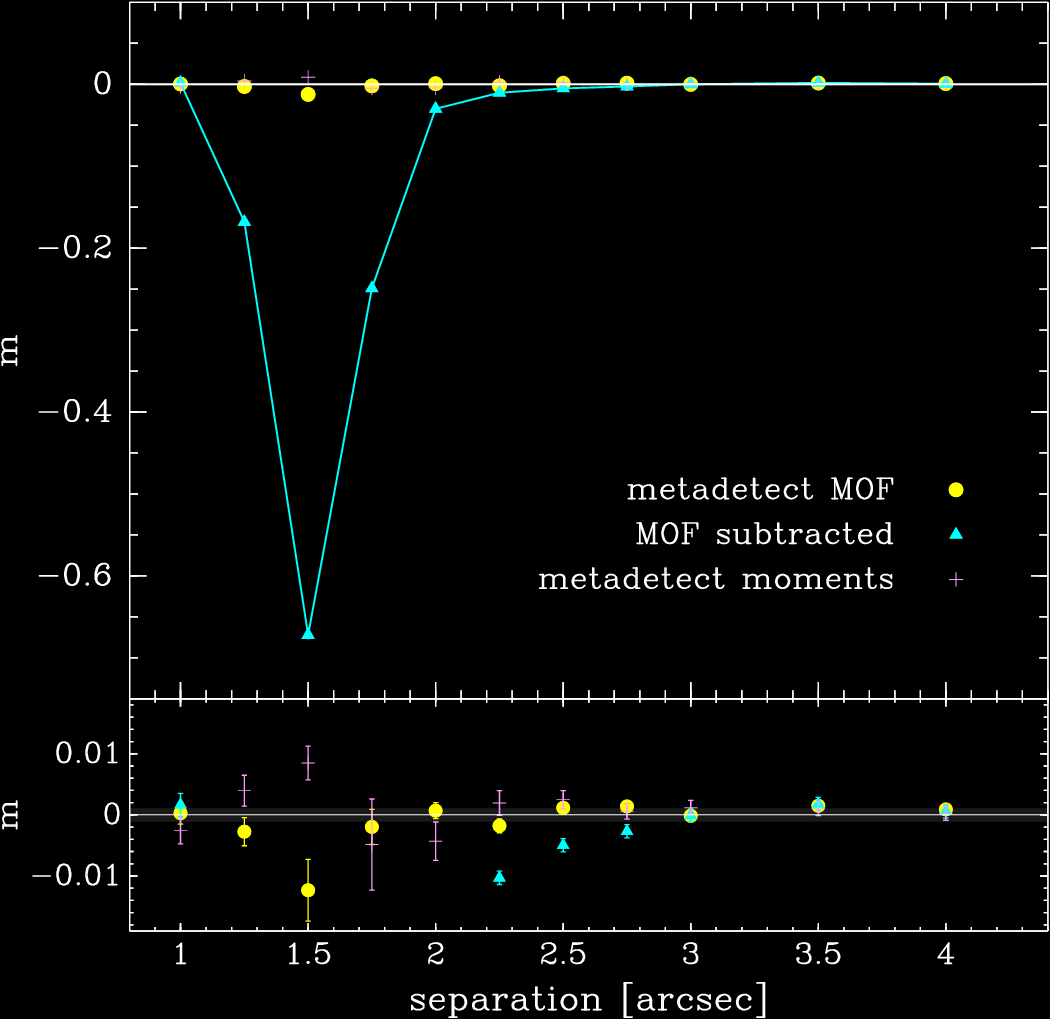
\includegraphics[width=\columnwidth]{pairs-mc-bdkpair-negate.png}
            \end{center}
        \end{column}
    \end{columns}
\end{frame}

\begin{frame}
    \frametitle{Metacalibration results for pair test}

    \setbeamerfont*{itemize/enumerate body}{size=\small}
    \setbeamerfont*{itemize/enumerate subbody}{parent=itemize/enumerate body}
    \setbeamerfont*{itemize/enumerate subsubbody}{parent=itemize/enumerate body}
 
    \begin{columns}
        \begin{column}{0.4\textwidth}
            \begin{itemize}

                \item Interpret as a {\color{lightsteelblue} shear-dependent detection bias}.

                \item We can mitigate the effect empirically; I will explain
                    the other symbols later.

            \end{itemize}
        \end{column}
        \begin{column}{0.6\textwidth}
            \begin{center}
                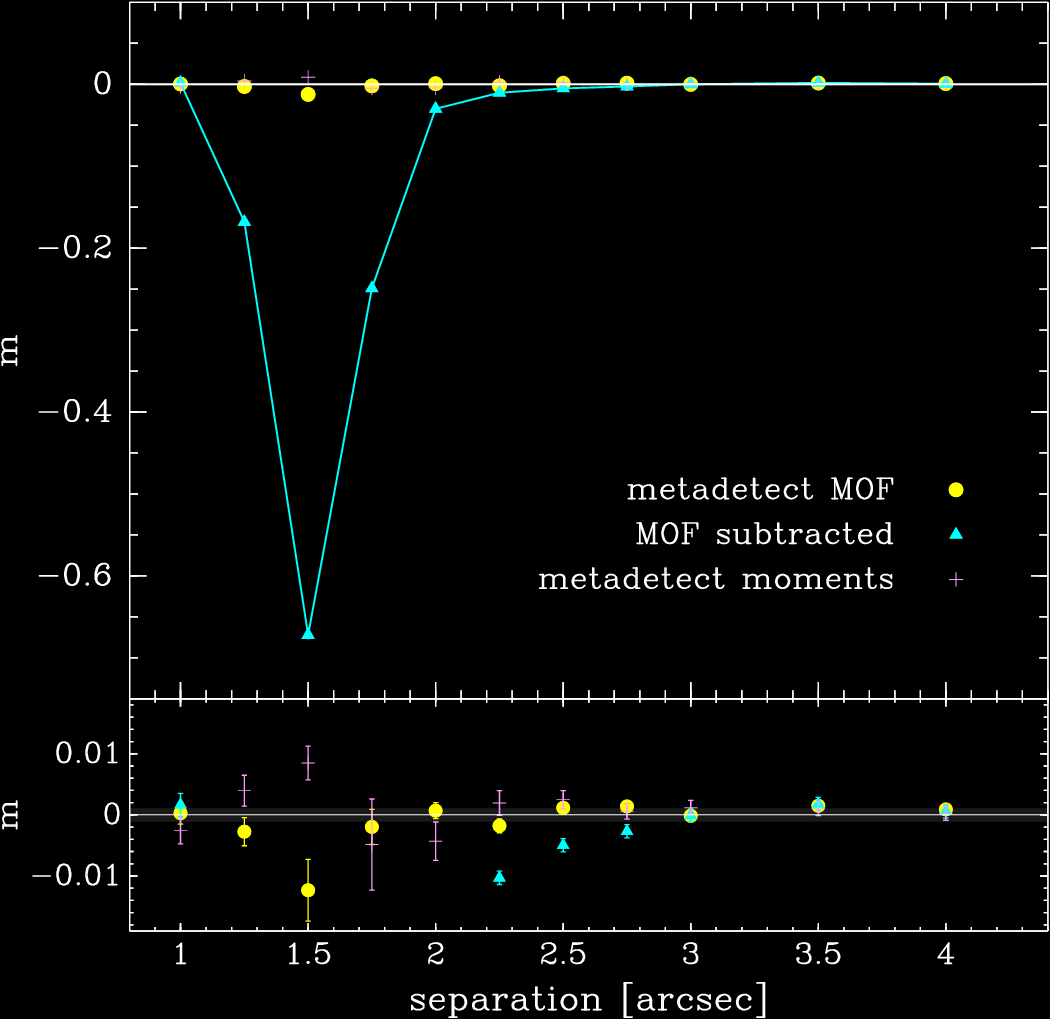
\includegraphics[width=\columnwidth]{pairs-mc-bdkpair-negate.png}
            \end{center}
        \end{column}
    \end{columns}
\end{frame}


\frame
{
    \frametitle{More Realistic Tests}

    \setbeamerfont*{itemize/enumerate body}{size=\normalsize}
    \setbeamerfont*{itemize/enumerate subbody}{parent=itemize/enumerate body}
    \setbeamerfont*{itemize/enumerate subsubbody}{parent=itemize/enumerate body}
 
    \begin{itemize}

        \item Same object types and survey parameters as the pair tests.

        \item Distribution of flux and size taken from the COSMOS $i<25.2$ catalog
            that comes with Galsim.
            \begin{itemize}
                \item Note this catalog lacks large bright galaxies. See images
                    on the next page.
            \end{itemize}

        \item \Mcal\ is unbiased for models with these properties when they
            appear individually.

        \item Noise appropriate for DES Y5

        \item {\color{lightsteelblue} sim1}: \neff={\color{green} 10}/sq arcmin for $S/N > 10$ and $T/T_{PSF} > 0.5$
            
        \item {\color{lightsteelblue} sim2}: \neff={\color{brightred} 35}/sq arcmin for $S/N > 10$ and $T/T_{PSF} > 0.5$.
            LSST-like density, but still used DES pixel and seeing (mistake)
            and I had to ``fake'' the catalog to go deeper.


    \end{itemize}

}

\frame
{
    \frametitle{Using the WeakLensingDeblending Package}

    \setbeamerfont*{itemize/enumerate body}{size=\normalsize}
    \setbeamerfont*{itemize/enumerate subbody}{parent=itemize/enumerate body}
    \setbeamerfont*{itemize/enumerate subsubbody}{parent=itemize/enumerate body}
 
    \begin{itemize}

        \item Using this package as a library.

        \item Shearing the entire scene, rather than shearing each object
            and then placing it which is how WeakLensingDeblending
            draws images.
            
        \item This way the positions also move, which is what happens
            during the \mcal\ shearing operations.

        \item I only have limited results in this configuration.

    \end{itemize}

}


\begin{frame}
    \frametitle{More realistic sims}
 
    \begin{columns}
        \begin{column}{0.5\textwidth}
            \begin{center}
                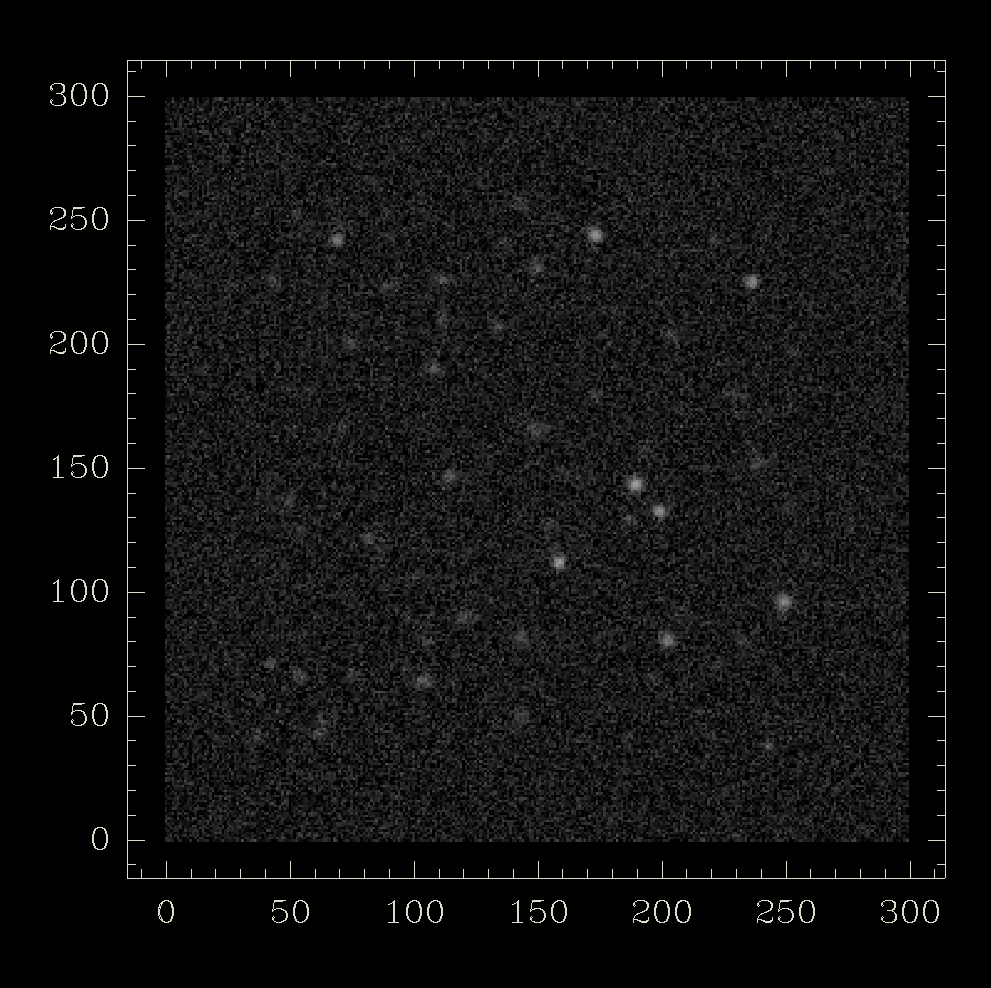
\includegraphics[width=\columnwidth]{10persqarcmin.png}
                \newline
                \neff=10/sq. arcmin
            \end{center}
        \end{column}
        \begin{column}{0.5\textwidth}
            \begin{center}
                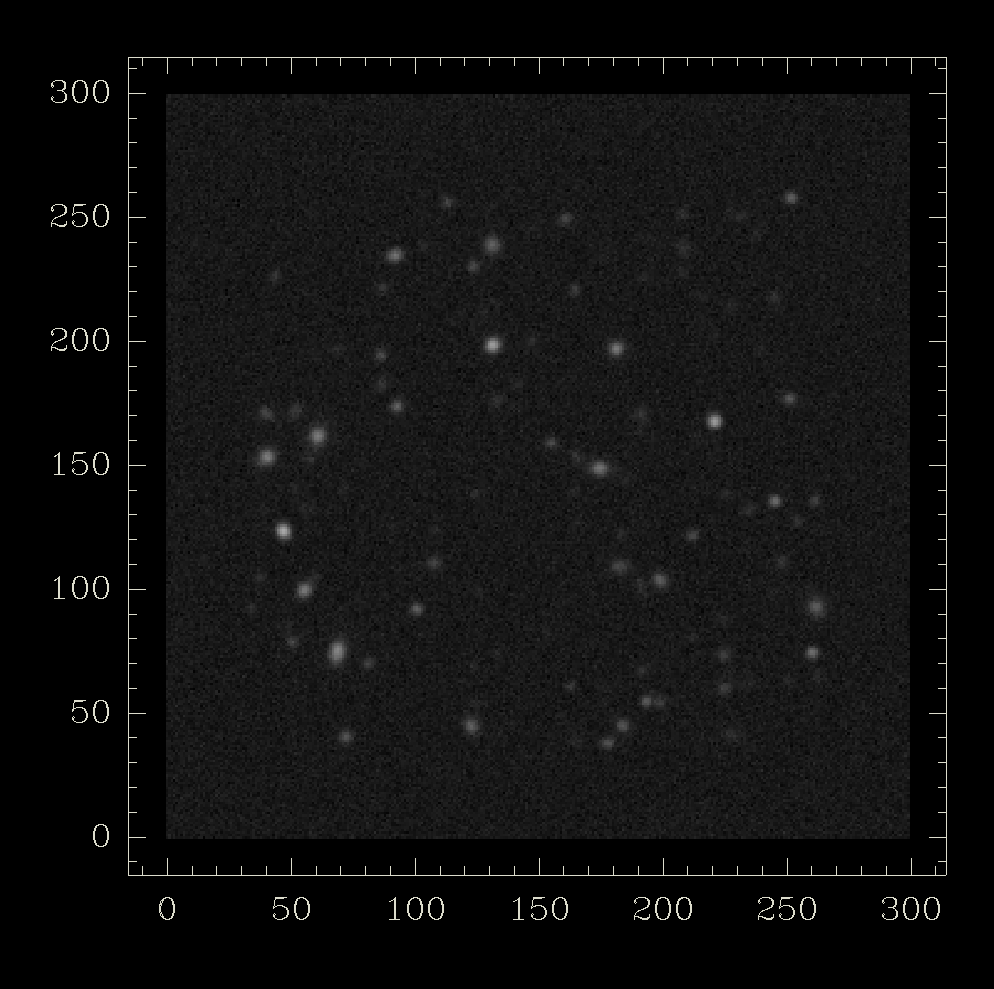
\includegraphics[width=\columnwidth]{35persqarcmin.png}
                \newline
                \neff=35/sq. arcmin
            \end{center}
        \end{column}
    \end{columns}
\end{frame}

\begin{frame}
    \frametitle{WeakLensingDeblending Sims}
 
    \begin{center}
        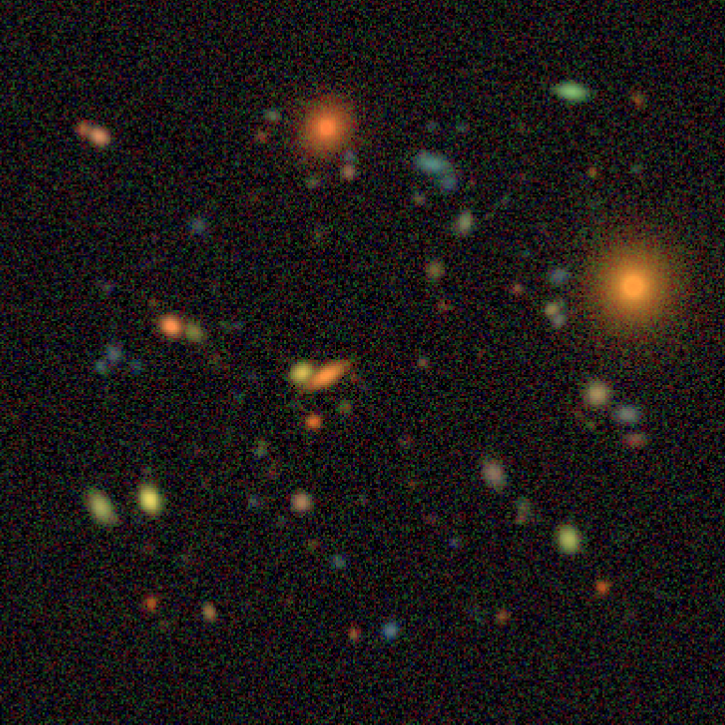
\includegraphics[height=0.75\textheight]{descwl-example1.png}
        \newline
        \neff=35/sq. arcmin
    \end{center}

\end{frame}



\begin{frame}
    \frametitle{Metacalibration results for more realistic sims}

    \setbeamerfont*{itemize/enumerate body}{size=\small}
    \setbeamerfont*{itemize/enumerate subbody}{parent=itemize/enumerate body}
    \setbeamerfont*{itemize/enumerate subsubbody}{parent=itemize/enumerate body}
 
    \begin{table}
        \centering
        \begin{tabular}{|l|l|c|c|}
            \hline
            Sim & Method         & \snr\ Cut & m             \\
            %    &          &           & $[10^{-2}]$   \\
            \hline

            \hline
            \neff={\color{green} 10} & MOF+metacal    & \snr$ > 10$ & $-0.016 \pm 0.003$  \\
            \neff={\color{green} 10} & MOF+metacal    & \snr$ > 15$ & $-0.038 \pm 0.003$  \\
            \neff={\color{green} 10} & MOF+metacal    & \snr$ > 20$ & $-0.053 \pm 0.003$  \\
            \hline
            %\neff={\color{brightred}35}  & uberseg+metacal    & \snr$ > 10$ & $-0.061 \pm 0.002$  \\
            %\neff={\color{brightred}35}  & uberseg+metacal    & \snr$ > 15$ & $-0.054 \pm 0.002$  \\
            %\neff={\color{brightred}35}  & uberseg+metacal    & \snr$ > 20$ & $-0.048 \pm 0.002$  \\
            \neff={\color{brightred}35}  & MOF+metacal    & \snr$ > 10$ & $-0.131 \pm 0.005$  \\
            \neff={\color{brightred}35}  & MOF+metacal    & \snr$ > 15$ & $-0.124 \pm 0.005$  \\
            \neff={\color{brightred}35}  & MOF+metacal    & \snr$ > 20$ & $-0.149 \pm 0.005$  \\
            \hline


        \end{tabular}
        \caption{Bias in more realistic simulations.  In all cases a cut
            of $T/T_{PSF} > 0.5$ was also applied.  The full MOF was not
            run for the \neff=35 sim due to lack of time.  Note the uberseg+metacal
            results generally agree with the MOF+metacal results for these
            sims.

        \label{tab:mcal:deblending}}
    \end{table}


\end{frame}


\frame
{
    \frametitle{Including Detection in the \mcal\ process}

    \setbeamerfont*{itemize/enumerate body}{size=\normalsize}
    \setbeamerfont*{itemize/enumerate subbody}{parent=itemize/enumerate body}
    \setbeamerfont*{itemize/enumerate subsubbody}{parent=itemize/enumerate body}
 
    \begin{itemize}

        \item There is a {\color{lightsteelblue} shear-dependent detection bias}.

        \item By bias, I mean everything that is done to find detections,
            not just determining what is above threshold.

        \item We can use \mcal\ to mitigate these effects. It involves
            creating the sheared images {\color{lightsteelblue} {\em before detection}}.

        \item The program:
            \begin{enumerate}

                \item Make the 5 \mcal\ images of a region of sky (not just for
                    one object).

                \item Run detection on each those to get 5 catalogs.

                \item Perform a measurement algorithm for each object.  This
                    could include deblending.

                \item Calculate the shear (or whatever statistic) using {\em
                    each} of the 5 catalogs.  The 4 sheared versions are used
                    to calculate the response, including detection effects.

            \end{enumerate}

    \end{itemize}

}

\begin{frame}
    \frametitle{Pair test including detection in the \mcal\ process}

    \setbeamerfont*{itemize/enumerate body}{size=\scriptsize}
    \setbeamerfont*{itemize/enumerate subbody}{parent=itemize/enumerate body}
    \setbeamerfont*{itemize/enumerate subsubbody}{parent=itemize/enumerate body}
 
    \begin{columns}
        \begin{column}{0.4\textwidth}
            \begin{itemize}

                \item The yellow circles represent results with deblending.
                The bias is greatly reduced, even at separations where
                    detection is highly uncertain.

                \item The magenta pluses represent results without deblending, just
                    measuring moments at the detected location using a circular
                    Gaussian weight function.

                \item The results are {\color{lightsteelblue} equally good
                    without deblending}.  This indicates that the biases come
                    from shear-dependent detection  not shear-dependent
                    deblending.

            \end{itemize}
        \end{column}
        \begin{column}{0.6\textwidth}
            \begin{center}
                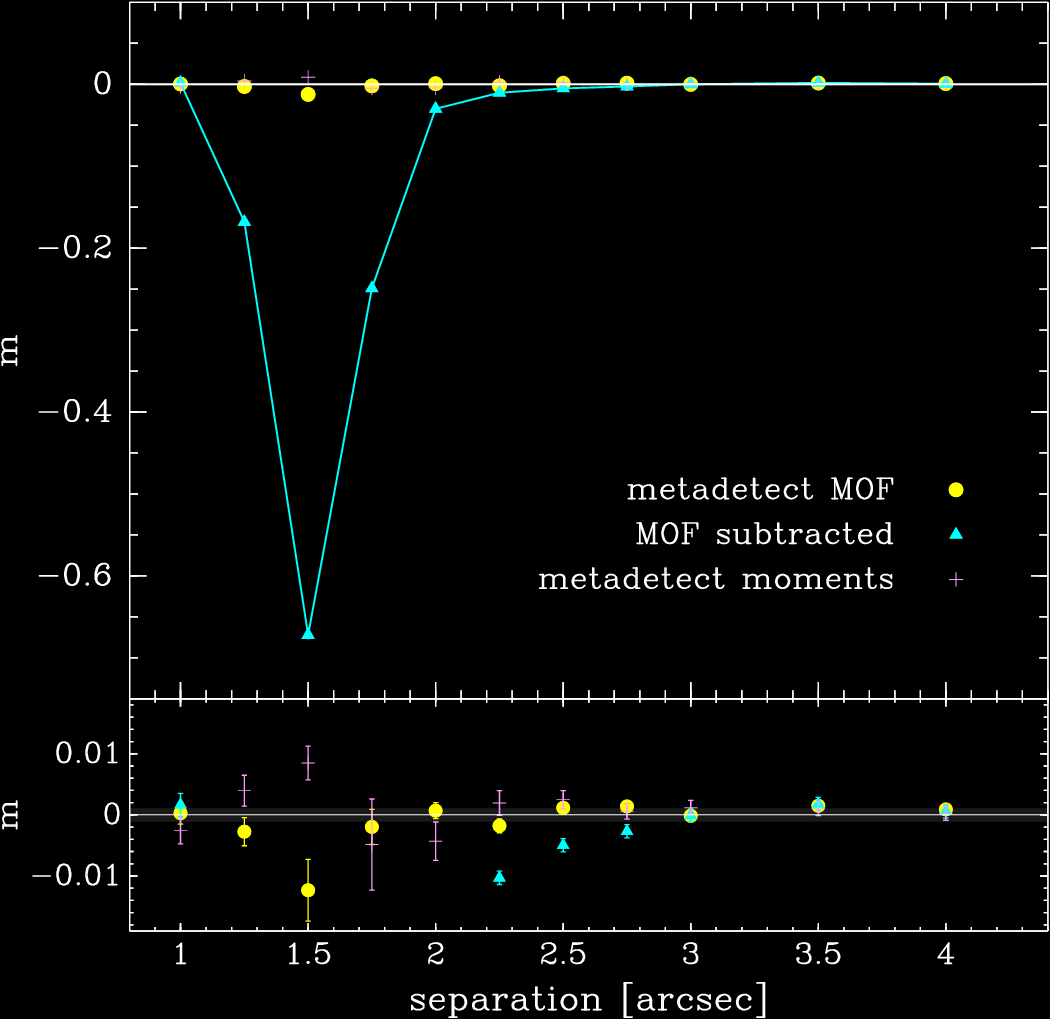
\includegraphics[width=\columnwidth]{pairs-mc-bdkpair-negate.png}
            \end{center}
        \end{column}
    \end{columns}
\end{frame}




\begin{frame}
    \frametitle{\Mcal\ detection results on more realistic sims.}

    \setbeamerfont*{itemize/enumerate body}{size=\small}
    \setbeamerfont*{itemize/enumerate subbody}{parent=itemize/enumerate body}
    \setbeamerfont*{itemize/enumerate subsubbody}{parent=itemize/enumerate body}
 
    \begin{table}
        \centering
        \begin{tabular}{|l|l|c|c|}
            \hline
            Sim & Method         & \snr\ Cut & m             \\
            %    &          &           & $[10^{-2}]$   \\
            \hline

            \hline
            \neff={\color{green} 10} & metadetect+MOF    & \snr$ > 10$ & $0.002 \pm 0.001$  \\
            \neff={\color{green} 10} & metadetect+MOF    & \snr$ > 15$ & $0.001 \pm 0.001$  \\
            \neff={\color{green} 10} & metadetect+MOF    & \snr$ > 20$ & $0.003 \pm 0.002$  \\
            \hline

        \end{tabular}
        \caption{Bias in more realistic simulations when \mcal\ includes
            the detection phase.  Deblending was performed using MOF. 
            In all cases a cut of $T/T_{PSF} > 0.5$ was also applied.
        \label{tab:mcal:deblending}}
    \end{table}


\end{frame}


\begin{frame}
    \frametitle{\Mcal\ detection results on more realistic sims without deblending.}

    \setbeamerfont*{itemize/enumerate body}{size=\small}
    \setbeamerfont*{itemize/enumerate subbody}{parent=itemize/enumerate body}
    \setbeamerfont*{itemize/enumerate subsubbody}{parent=itemize/enumerate body}
 
    \begin{table}
        \centering
        \begin{tabular}{|l|l|c|c|}
            \hline
            Sim & Method         & \snr\ Cut & m             \\
            %    &          &           & $[10^{-2}]$   \\
            \hline

            \hline
            \neff={\color{green} 10} & metadetect+moments    & \snr$ > 10$ & $+0.0001 \pm 0.0014$  \\
            \neff={\color{green} 10} & metadetect+moments    & \snr$ > 15$ & $-0.0002 \pm 0.0017$  \\
            \neff={\color{green} 10} & metadetect+moments    & \snr$ > 20$ & $-0.0037 \pm 0.0025$  \\
            \hline
            \neff={\color{brightred}35}    & metadetect+moments    & \snr$ > 10$ & $-0.0002 \pm 0.0008$  \\
            \neff={\color{brightred}35}    & metadetect+moments    & \snr$ > 15$ & $-0.0009 \pm 0.0008$  \\
            \neff={\color{brightred}35}    & metadetect+moments    & \snr$ > 20$ & $-0.0005 \pm 0.0008$  \\
            \hline

        \end{tabular}
        \caption{Bias in more realistic simulations when \mcal\ includes
            the detection phase.  No deblending was performed, 
            moments were measured using a circular Gaussian weight function.
            In all cases a cut of $T/T_{PSF} > 0.5$ was also applied.
        \label{tab:mcal:deblending}}
    \end{table}


\end{frame}


\begin{frame}
    \frametitle{\Mcal\ detection results on WeakLensingDeblending sims.}

    \setbeamerfont*{itemize/enumerate body}{size=\small}
    \setbeamerfont*{itemize/enumerate subbody}{parent=itemize/enumerate body}
    \setbeamerfont*{itemize/enumerate subsubbody}{parent=itemize/enumerate body}
 
    \begin{table}
        \centering
        \begin{tabular}{|l|l|c|c|}
            \hline
            Sim & Method         & \snr\ Cut & m             \\
            %    &          &           & $[10^{-2}]$   \\
            \hline

            \hline
            \neff={\color{brightred}35}    & metadetect+moments    & \snr$ > 10$ & $XXX \pm XXX$  \\
            \neff={\color{brightred}35}    & metadetect+moments    & \snr$ > 15$ & $XXX \pm XXX$  \\
            \neff={\color{brightred}35}    & metadetect+moments    & \snr$ > 20$ & $XXX \pm XXX$  \\
            \hline

        \end{tabular}
        \caption{Bias in LSST WeakLensingDeblending simulations when \mcal\ includes
            the detection phase.  No deblending was performed, 
            moments were measured using a circular Gaussian weight function.
            In all cases a cut of $T/T_{PSF} > 0.5$ was also applied.
        \label{tab:mcal:deblending}}
    \end{table}


\end{frame}

\begin{frame}
    \frametitle{\Mcal\ detection results on WeakLensingDeblending sims.}

    \begin{itemize}

        \item I also ran the WeakLensingDeblending simulation where I shear the
            objects ``in place'', one at a time rather than shearing the entire
            scene, 

        \item I saw biases as large as -1\%, but it depended on the cuts
            applied.  This dependence implies the detection effects are not
            being corrected.

        \item Real galaxies are at different redshifts, so it is some kind of
            ``hybrid'' where different parts of the scene are all sheared
            together.

        \item Should try to simulate that.

    \end{itemize}



\end{frame}





\frame
{
    \frametitle{Challenges for Real Data}

    \setbeamerfont*{itemize/enumerate body}{size=\small}
    \setbeamerfont*{itemize/enumerate subbody}{parent=itemize/enumerate body}
    \setbeamerfont*{itemize/enumerate subsubbody}{parent=itemize/enumerate body}
 
    \begin{itemize}

        %\item Requires calculating the statistic of interest 5 times, once for
        %    each catalog. Should not be a problem.

        \item Must identify regions of sky large enough for
            good detection and for which the PSF is approximately constant.
            e.g. 1x1 arcminute patches.

        \item Must deal with parts of the image that cannot be deconvolved. For
            example effects that occur in the detector such as bad pixels, bleed trails
            from bright stars, cosmic rays, etc.

        \item Must merge catalogs from between the different patches, so
            the patches should include some padding.  We need to test if this
            merging causes shear dependent selection effects.

        \item We need a continuous PSF, so we need these coadds to be made
            excluding images that have a boundary in the region of interest.
            We generally call these ``coadds in cells''.
            See Jim  Bosche's talk on coadds and my talk on coadds.

        \item Objects are at different redshifts, so we will need to be a bit
            smarter about the \mcal\ image shearing to avoid potential
            percent level biases.

    \end{itemize}

}



%\frame
%{
%    \frametitle{Fluxes: comparison of formula with simulation}
 
%        %\newline
%        $\Delta \sigma_p/\sigma_p = 0.10$
%    \begin{center}
%        \colorbox{white}{
%            \includegraphics[width=\columnwidth]{{cnoise-fwhm0.90-frac0.10-ntrial100000}.pdf}
%        }
%        \newline
%        (Sheldon, Armstrong, Huff, et al. in prep)
%    \end{center}


%}


\end{document}
